\documentclass[11pt]{amsart}
\usepackage{geometry}                % See geometry.pdf to learn the layout options. There are lots.
\geometry{letterpaper}                   % ... or a4paper or a5paper or ... 
%\geometry{landscape}                % Activate for for rotated page geometry
%\usepackage[parfill]{parskip}    % Activate to begin paragraphs with an empty line rather than an indent
\usepackage{graphicx}
\usepackage{subfigure}
\usepackage{amssymb}
\usepackage{epstopdf}
\DeclareMathOperator*{\argminA}{arg\,min} % Jan Hlavacek
\DeclareMathOperator*{\argminB}{argmin}   % Jan Hlavacek
\DeclareMathOperator*{\argminC}{\arg\min}   % rbp

\newcommand{\argminD}{\arg\!\min} % AlfC

\newcommand{\argminE}{\mathop{\mathrm{argmin}}}          % ASdeL
\newcommand{\argminF}{\mathop{\mathrm{argmin}}\limits}   % ASdeL

% limits on side
\DeclareMathOperator{\argminG}{arg\,min} % Jan Hlavacek
\DeclareMathOperator{\argminH}{argmin}   % Jan Hlavacek
\newcommand{\argminI}{\mathop{\mathrm{argmin}}\nolimits} % ASdeL

\newcommand{\cs}[1]{\texttt{\symbol{`\\}#1}}
\DeclareGraphicsRule{.tif}{png}{.png}{`convert #1 `dirname #1`/`basename #1 .tif`.png}
\geometry{left=2cm,right=2cm}
\title{ Reinforcement learning in financial computing}
%\author{The Author}
%\date{}                                           % Activate to display a given date or no date

\begin{document}
\maketitle
%\section{}
%\subsection{}

\section{DQN}
Although the previous algorithms work well in low dimensions, solving high-dimensional HJB is our goal. Due to the difficult problem known as the ''curse of dimensionality'', as the dimension grows, neither value iteration nor Q-learning can return a result in a limited time. Inspired by DeepBSDE$^{1}$ and AlhphaGO$^{2}$, deep reinforcement learning could be a solution to solve the high-dimensional HJB problems.
\subsection{Basic DQN}
We want to test the effect of deep learning algorithm on low dimension.
\subsubsection{Methodology}

Consider the deep neural network as a nolinear function $h$, what we want to do is train the network so that for each input, it can return a value close to the exact solution.  For the d-dimensions HJB given below
\begin{itemize}
 \item Domain 
 $$O = \{x\in \mathbb R^{d}: 0<x_{i}< 1, i =1,2, \ldots d\}.$$
 \item Equation on $O$: 
 $$(\frac 1 2 \Delta -  \lambda) v(x) + \inf_a \Big\{
 \sum_{i=1}^db_i(x,a)  \frac{\partial v(x)}{\partial x_i}  
  + \ell(x,a)
 \Big\} = 0.$$
 \item Dirichlet data on $\partial O$:
 $$v(x) = g(x).$$
Where $v(x)$ is the exact solution for this problem and $g(x),b_i(x) , \ell(x)$ are known functions.
\end{itemize}
As we mentioned before, if we introduce some notions of finite difference operators on HJB, it yields DPP:
$$
v (x) = \gamma \inf_{a} 
\Big\{ \ell^{h}(x, a) + 
\sum_{i=1}^{d} 
p^{h}(x+he_{i}|x, a) v(x+he_{i})
+ p^{h}(x-he_{i}|x, a) v(x-he_{i})
\Big\}.
$$
where $\ell^{h}(x),p^{h}(x \pm he_{i}|x),\gamma $ are known.
\\ \hspace*{\fill} \\
In value iteration or Q-learning, what we have done is actually giving all $g(x)$ an initial value and then make all the values converge to the exact solution by iterating the above formula. In fact, that's why these algorithms can't be extended to high-dimensional HJB problems: it is impossible to iterate all the points in high dimensional space. While in value iteration or Q-learning algorithms, all points are associated with each other. If we can't iterate, all the values are meaningless. 
\\ \hspace*{\fill} \\
In this section, we turn the focus from getting the numerical solution of HJB to getting HJB function itself (Even though our results is a black box and unwritable). This will give us the possibility of calculation in the case of high dimension. Briefly, we are going to use deep neural network to simulate the exact HJB function. 
\\ \hspace*{\fill} \\
For a certain input, we have two ways to get its value $v(x)$ through neural network, one comes directly from the neural network, and the other is obtained by combining DPP formula with network:
$$
v(x) = h(x,\theta)
$$
$$
v(x)  = \gamma \inf_{a} 
\Big\{ \ell^{h}(x, a) + 
\sum_{i=1}^{d} 
p^{h}(x+he_{i}|x, a) h(x+he_{i} ,\theta)
+ p^{h}(x-he_{i}|x, a) h(x-he_{i} ,\theta)
\Big\}. 
$$
Where $\theta$ is the set of parameters in the neural network.\\
Ideally, if the deep neural network can return values close to the exact solutions, they should be equal. So our goal is to find the specific parameters that make the difference between them as small as possible:
$$
\argminA_\theta\Big \{h(x,\theta) - \gamma \inf_{a} 
\Big\{ \ell^{h}(x, a) + 
\sum_{i=1}^{d} 
p^{h}(x+he_{i}|x, a) h(x+he_{i} ,\theta)
+ p^{h}(x-he_{i}|x, a) h(x-he_{i} ,\theta)\Big\}\Big\}
$$
Based on this formula, we can define the loss function $L$ for our network:
$$
L(\theta) = \sum_{i=1}^{N} {\argminA_\theta\Big \{h(x_i,\theta) - \gamma \inf_{a} 
\Big\{ \ell^{h}(x, a) + 
\sum_{i=1}^{d} 
p^{h}(x+he_{i}|x, a) h(x_i+he_{i} ,\theta)
+ p^{h}(x-he_{i}|x, a) h(x_i-he_{i} ,\theta)\Big\}\Big\}}
$$
\\ \hspace*{\fill} \\
\subsubsection{Examples} 
Multidimensional HJB with quadratic function as its solution.\\
Consider:
$$
 \frac 1 2 \Delta v + \inf_{a\in \mathbb R^{d}}
 \Big(a \cdot \nabla v +d + 2|x|^2 + \frac 1 2 |a| ^2 \Big) = 0, \ x\in O.
$$
with
$$
v(x) = -|x|^2, \ x\in \partial O.
$$
The exact solution is 
$$
v(x) =  -|x|^2, \ \hbox{ with } a= 2x.
$$
This means that the solution is invariant if $\inf_{a\in \mathbb R^{d}}$ is
replaced by $\inf_{a\in 3 O}$
\\ \hspace*{\fill} \\
\subsubsection{Implementation} We build a neural network to test the effect of deep learning algorithm in low dimension. This neural work is fully connected and consists of four layers, with one input layer ($d$ dimensional), two hidden layers (both 2*$d$+10 dimensional), and one output layer (1 dimensional). We choose the rectifier function(ReLU) as our activation function. For the example above in 2 dimensions, after 100 iterations and then compare the result of neural network with the exact solution, the sup norm error is: 0.2678.

\begin{figure}[htbp]
\centering
\subfigure[Neural Network Result]{
\begin{minipage}[t]{0.5\linewidth}
\centering
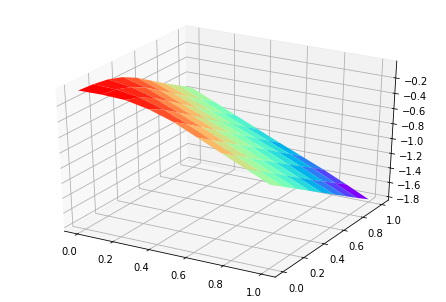
\includegraphics[width=3in]{5_1network.jpg}
%\caption{fig1}
\end{minipage}%
}%
\subfigure[Exact Solution]{
\begin{minipage}[t]{0.5\linewidth}
\centering
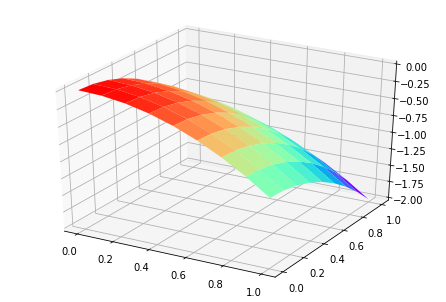
\includegraphics[width=3in]{5_1exact.jpg}
%\caption{fig2}
\end{minipage}%
}%
\centering
\caption{ 2-dimensional HJB}
\end{figure}


\subsubsection{Conclusion and Problems}
\begin{itemize}
 \item Construction of neural network\\
If the constructed neural network is regarded as a set of functions, then only if the exact solution is in the set can we get a good result. Actually, in the beginning, we used a simple neural network to try to solve the 1-$d$ HJB and failed. So how to build a neural network to make the exact solution included in the neural network is an important problem.
 \item Construction of loss function\\
Since we knew the Boundary value at the beginning, so we hope that the results of the neural network on boundary can be as correct as possible. Then we changed the loss function to:

$$ L^{'}(\theta) =\left\{
\begin{aligned}
&L(\theta),\ x_i  \notin \partial O\\
&W*\argminA_\theta [v(x)-h(x,\theta)]^2 ,\ x_i \in \partial O
\end{aligned}
\right.
$$
Where $W$ is the weight we set to improve the accuracy in boundary. Actually, without the weight, we may get a result similar to the exact solution but different in the boundary.
 \item Performance\\
Although neural network could give us a result, both the accuracy and the calculation time are worse than Q-learning and value iteration. How to improce its efficiency can be a direction.
\end{itemize}



\end{document}  